\chapter{Задание}

Разработать программное обеспечение, предоставляющее возможность вычислить предельные вероятности состояний и среднее время нахождения в каждом состоянии для сложной системы в установившемся режиме работы с числом состояний $\leq 10$.

Интерфейс должен позволять указать число состояний и ввести матрицу интенсивностей потоков переходов состояний. В результате работы алгоритма должны быть отображены предельные вероятности и среднее время нахождения системы в каждом из состояний.
\chapter{Теоретическая часть}
\section{Марковский процесс}
Случайный процесс, протекающей в некоторой сложной системе, называется марковским, если для каждого момента времени $t$ вероятность любго состояни системы в будущем зависит только от состояния в настоящем и не зависит от того, когда и каким образом система пришла в это состояние.

Процесс, протекающий в системе, которая может находиться в одном из $n$ состояний, задается матрицей интенсивностей потоков переходов, которая имеет вид:
\begin{equation}
    \begin{pmatrix}
        \lambda_{1, 1} & \lambda_{1, 2} & \dots & \lambda_{1, j} & \dots &\lambda_{1, n}\\
        \lambda_{2, 1} & \lambda_{2, 2} & \dots & \lambda_{2, j} & \dots &\lambda_{2, n}\\
        \vdots & \vdots & \ddots &\vdots &\ddots &\vdots\\
        \lambda_{i, 1} & \lambda_{i, 2} & \dots & \lambda_{i, j} & \dots &\lambda_{i, n}\\
        \vdots & \vdots & \ddots &\vdots &\ddots &\vdots\\
        \lambda_{n, 1} & \lambda_{n, 2} & \dots & \lambda_{n, j} & \dots &\lambda_{n, n}\\
    \end{pmatrix},
\end{equation} 
где $\lambda_{i,j}$~---~интенсивность потока перехода из состояния $i$ в состояние $j$.

Для определения вероятности нахождения системы в некотором состоянии в момент времени $t$ составляют уравнения Колмогорова. Для сосостояния $i$ уравнение имеет вид:
\begin{equation}
    \label{eq:kolmogorov_i}
    p'_{i}(t) = \sum_{j=1}^{n} \lambda_{j,i}p_{j}(t) - p_{i}(t) \sum_{j=1}^{n}\lambda_{i,j},
\end{equation}
где $p_{i}(t)$~---~вероятность нахождения системы в состоянии $i$ в момент времени $t$.

\section{Вычисление предельных вероятностей нахождения в отдельно взятом состоянии}
При стационарном (установившемся) режиме работы ($t\rightarrow\infty$) системы, производные вероятностей состояний в~\ref{eq:kolmogorov_i} полагаются равными нулю. В этом случае, уравнения Колмогорова образуют систему линейных алгебраических уравнений вида:
\begin{equation}
    \begin{cases}
        \sum_{j=1}^{n} \lambda_{j,1}p_{j} - p_{1} \sum_{j=1}^{n}\lambda_{1,j} = 0 \\
        \sum_{j=1}^{n} \lambda_{j,2}p_{j} - p_{2} \sum_{j=1}^{n}\lambda_{2,j} = 0 \\
        \dots \\
        \sum_{j=1}^{n} \lambda_{j,n}p_{j} - p_{n} \sum_{j=1}^{n}\lambda_{n,j} = 0
    \end{cases}
\end{equation}
где $p_i$~---~предельная вероятность нахождения системы в состоянии $i$ при $t\rightarrow\infty$.

Полученная СЛАУ является однородной и в общем случае может не иметь нетривиального решения. Дополнительно вводится условие нормировки вида:
\begin{equation}
    \sum_{i=1}^{n}p_{i} = 1
\end{equation}

Для решения СЛАУ в программной реализации используется сингулярное разложение из математического пакета Eigen, которое позволяет найти правый сингулярный вектор, который представляет ненормированные корни однородной СЛАУ.

\section{Вычисление среднего времени нахождения в отдельно взятом состоянии}
Для вычисления среднего времени нахождения системы в состоянии $i$ используется выражение:
\begin{equation}
    t_i = \frac{p_i}{\sum_{j=1, j \ne i}^{n}(\lambda_{i, j}+\lambda_{j, i})+\lambda_{i, i}}
\end{equation}

\chapter{Практическая часть}
\section{Результаты работы программы}
Результаты работы программы представлены на рисунках~\ref{fig:res1}~\ref{fig:res2}.
\begin{figure}[H]
    \centering
    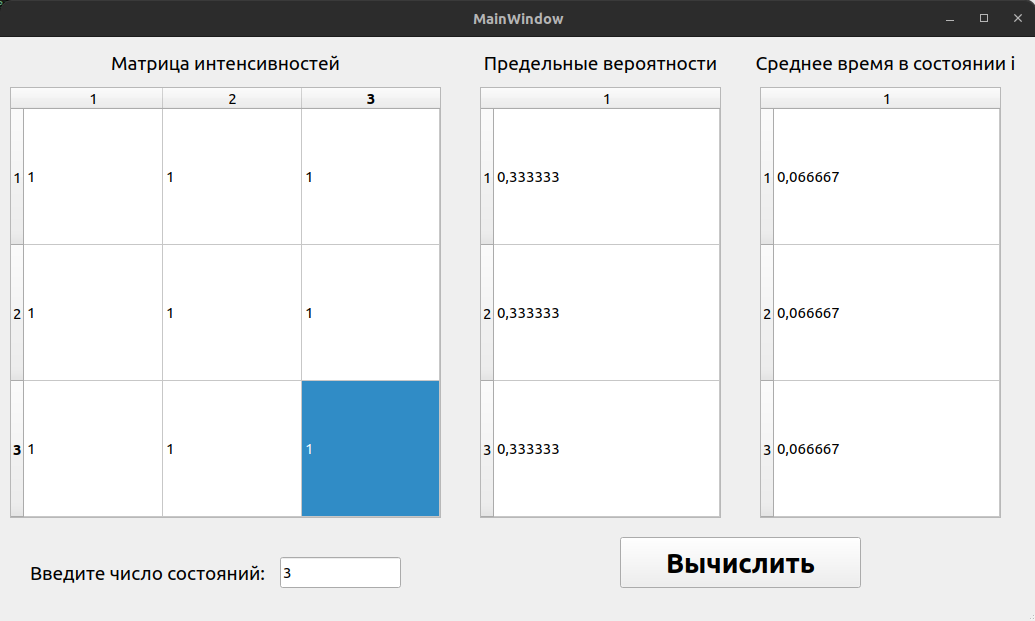
\includegraphics[width=0.9\linewidth]{images/example_1.png}
    \caption{Результат работы программы}
    \label{fig:res1}
\end{figure}
\begin{figure}[H]
    \centering
    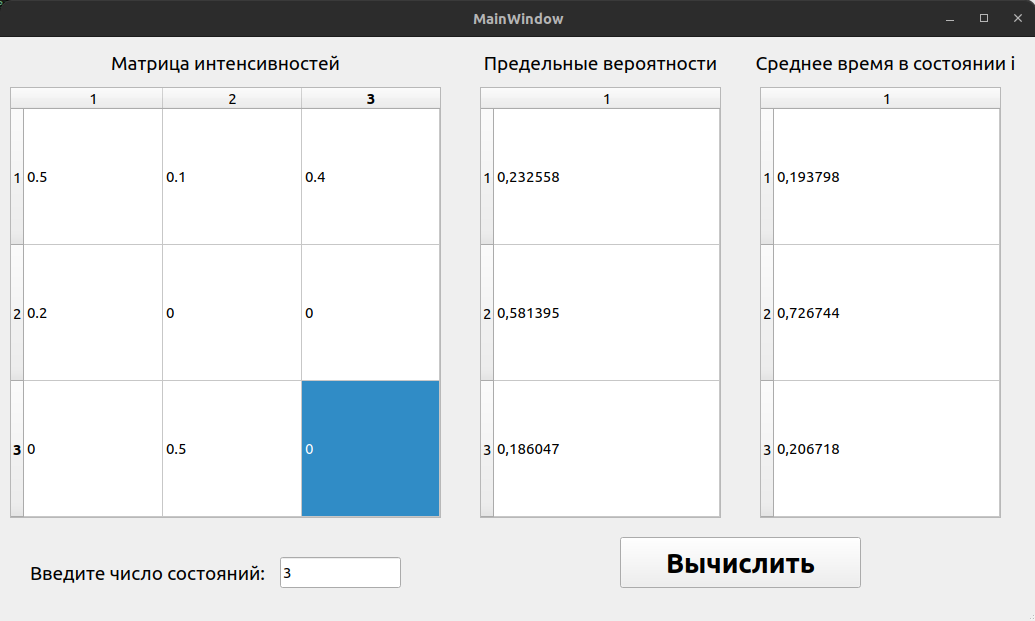
\includegraphics[width=0.9\linewidth]{images/example_2.png}
    \caption{Результат работы программы}
    \label{fig:res2}
\end{figure}